% !TeX program = pdflatex
\documentclass[russian,utf8,emptystyle,reduceheight=5mm]{eskdtext}

% packages
%
% Тестовое наполнение текстом
% При написании работы - удалить пакет и комманды \lipsum
\usepackage{lipsum}
%
\usepackage{eskdplain}
\usepackage{graphicx}
\usepackage{datetime}
\usepackage{enumitem} % for lists
\usepackage{ulem} % for underlining
\usepackage{lastpage} % Number of pages
\usepackage{hyperref} % Links in pdf

% setup
\newcommand{\FrontPageDepartment}{ЭМ} %Факультет
\newcommand{\FrontPageSubdepartment}{Менеджмента} %Кафедра
\newcommand{\WorkType}{Контрольная работа} %Тип работы (заголовок)
\newcommand{\Subject}{Предмет} %по ... родительный падеж
\newcommand{\Topic}{Тема контрольной работы} %Тема
\newcommand{\Professor}{Иванов~И.~И.} %Руководитель
\newcommand{\Student}{Петров~П.~П.} %Студент
\newcommand{\Group}{ИСм-112} %Группа
\newcommand{\FrontPageDate}{\ddmmyyyydate\today} %Дата

\ESKDsignature{МИВУ 230400.68 ПЗ} % Код специальности и тип работы

% eskdx setup
\ESKDletter{}{У}{}
\ESKDtitle{\Topic}
\ESKDchecker{\Professor}
\ESKDauthor{\Student}
\ESKDcolumnIX{МИ ВлГУ\\ \Group}

\addto\captionsrussian{\def\refname{Список использованных источников}}
\sloppy % split long lines

% eskdx setup
\ESKDletter{}{У}{}
\ESKDtitle{\Topic}
\ESKDchecker{\Professor}
\ESKDauthor{\Student}
\ESKDcolumnIX{МИ ВлГУ\\ \Group}

\addto\captionsrussian{\def\refname{Список использованных источников}}
\sloppy % split long lines

% graphics path
\graphicspath{{src/img/}}


% verbatim setup
\newcommand{\verbatimFont}{
\fontsize{10pt}{12pt}\selectfont
\baselineskip=1em
}


% workaround for regression in babel package on linux
\providecommand{\No}{\textnumero}


% remove vertical space from lists
\renewcommand{\alph}[1]{\asbuk{#1}} % костыль для кирилической нумерации вместо латинской
\setlist{nolistsep} % убираем дополнительные вертикальные отступы вокруг списков
\setenumerate[1]{label=\alph*), fullwidth, itemindent=\parindent,  listparindent=\parindent}
\setenumerate[2]{label=\arabic*), fullwidth, itemindent=\parindent, listparindent=\parindent, leftmargin=\parindent}
\setitemize{fullwidth, itemindent=\parindent, listparindent=\parindent}
\newlength{\PAGEborderLR}
\newlength{\PAGEborderTB}

\setlength{\PAGEborderLR}{2cm}
\setlength{\PAGEborderTB}{2cm}

% Set up page
\setlength{\hoffset}{-2.54cm + \PAGEborderLR}
\setlength{\voffset}{-2.54cm + \PAGEborderTB}
\setlength{\topskip}{0pt}
\setlength{\footskip}{21pt}
\setlength{\oddsidemargin}{0pt}
\setlength{\evensidemargin}{0pt}
\setlength{\topmargin}{0pt}
\setlength{\headheight}{0pt}
\setlength{\headsep}{0pt}
\setlength{\textwidth}{210mm-\PAGEborderLR*2}
\setlength{\textheight}{297mm-\PAGEborderTB*2-\footskip}
\setlength{\marginparsep}{0pt}
\setlength{\marginparwidth}{0pt}
\setlength{\marginparpush}{0pt}

% main document
\begin{document}
% Титул
\ESKDthisStyle{empty}
\setlength{\topskip}{15pt}
\thispagestyle{empty}

\pdfbookmark{Титульный лист}{FrontpagePdfBookmark}

\begin{center}
\baselineskip=12pt
{\normalsize Министерство образования и науки Российской Федерации}

\textbf{Муромский институт (филиал)}

{\small федерального государственного бюджетного образовательного учреждения}

{\small высшего профессионального образования}

\textbf{<<Владимирский государственный университет}

\textbf{\makebox[\textwidth]{имени Александра Григорьевича и Николая Григорьевича Столетовых>>}}

{\normalsize \textbf{(МИ (филиал) ВлГУ)}}
\end{center}

\vspace{\fill}

\begin{flushright}
На правах рукописи
\end{flushright}

\bigskip

\begin{center}
\textbf{\Author}

\vspace{\fill}

\textbf{\MakeUppercase{\thetitle}}
\end{center}

\vspace{\fill}

\begin{center}
\makebox[\textwidth]{Направление подготовки \Speciality}
\end{center}

\vspace{\fill}

\begin{center}
Магистерская диссертация
\end{center}

\vspace{\fill}

\begin{flushright}
Научный руководитель:

\ProfessorDegree

\Professor
\end{flushright}


\vspace{\fill}

\begin{center}
Муром --- \the\year
\end{center}
\setlength{\topskip}{0pt}
\newpage

% Аннотация
\ESKDthisStyle{empty}
\vspace*{\fill}
Курсовой проект посвящен разработке и реализации ...

В курсовом проекте подробно описано техническое задание, проведена разработка алгоритмов, программы, написано руководство, осуществлено тестирование системы.

Объём пояснительной записки составляет \pageref{LastPage} листов. Количество рисунков - 2 штуки. Таблицы отсутствуют.
\vspace*{\fill}
\newpage

% Содержание
\setcounter{page}{4}
\tableofcontents
\newpage

% Основной текст
\begin{center}
\textbf{Лабораторная работа №1}
\\
\textbf{Тема:} Работа с системами контроля версий
\\
\end{center}
\textbf{Задание:} 
\begin{enumerate}
\item Зарегистрироваться на https://github.com/
\item Склонировать репозиторий шаблонов tex https://github.com/egorpugin/tex;
\item Подготовить шаблон отчёта для лабораторных работ в LaTeX;
\item Загрузить шаблон в репозиторий tex;
\item Создать новый репозиторий для лабораторных работ на гитхабе;
\item Оформить отчёт и загрузить его в репозиторий для ЛР;
\\
\end{enumerate}
\begin{figure}[h]
\centering
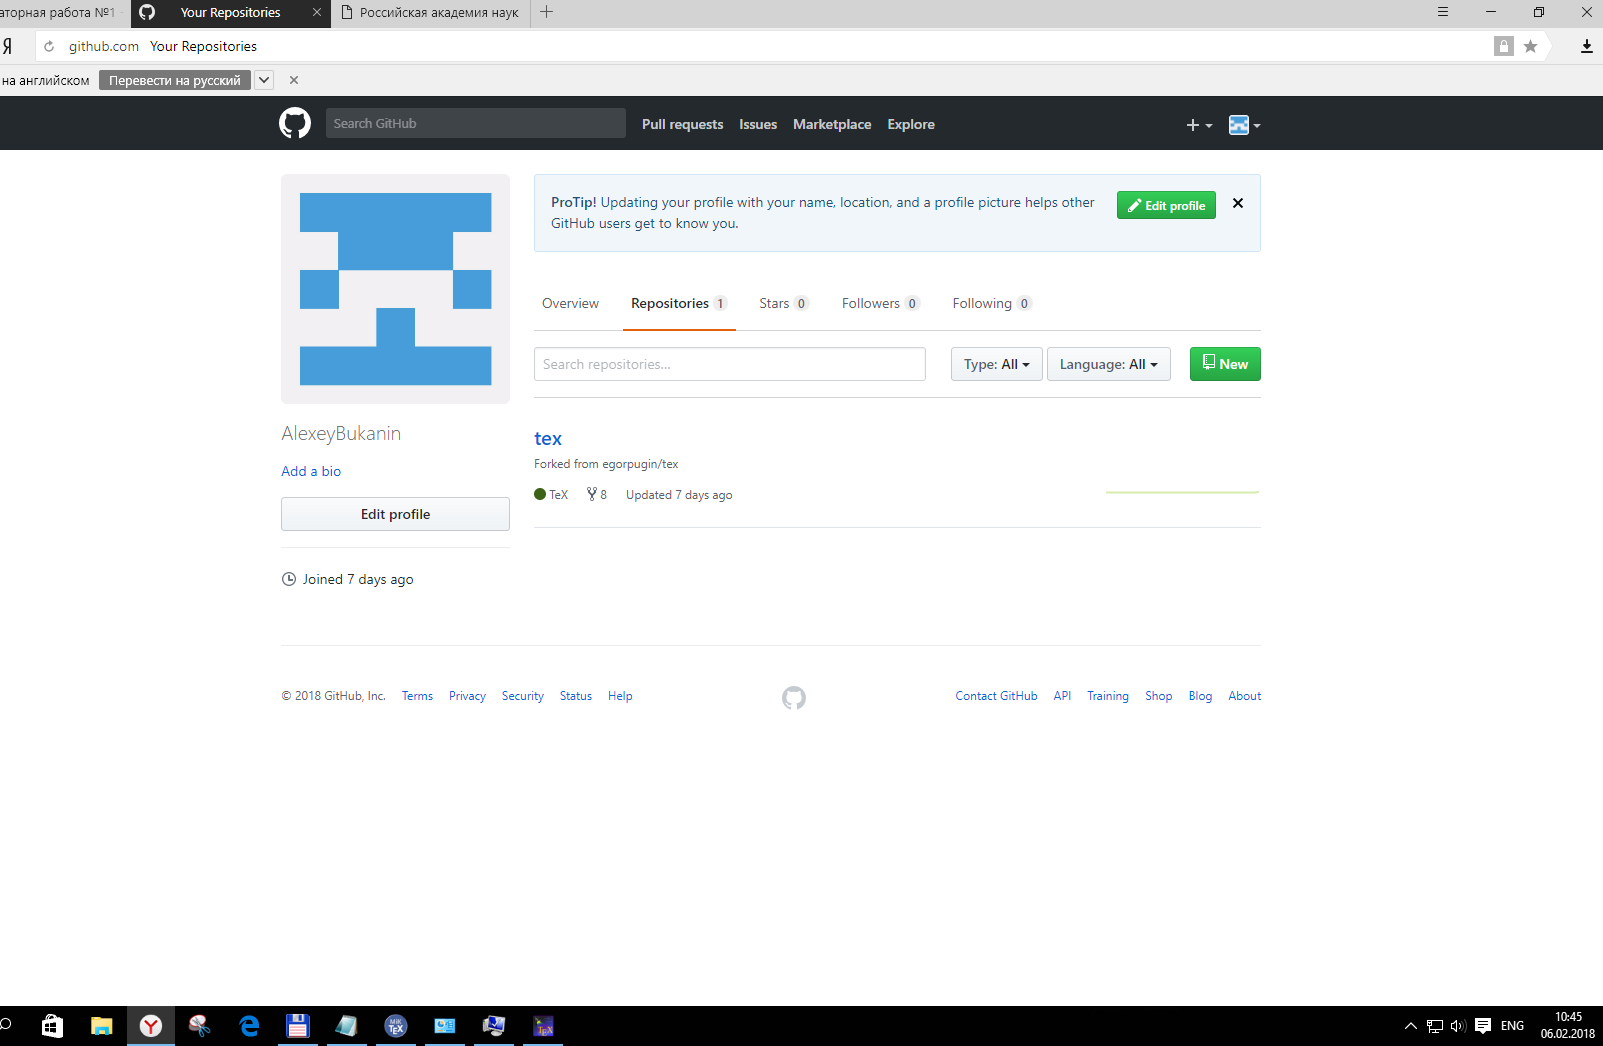
\includegraphics[scale=0.4]{repoz}
\caption{Сайт github.com}
\label{fig:repoz}
\end{figure}

\newpage
\begin{enumerate}
\item Создали репозиторий
\item Добавили файл
\item Зафиксировали изменения
\item Отправили на github

\end{enumerate}

\begin{figure}[h]
\centering
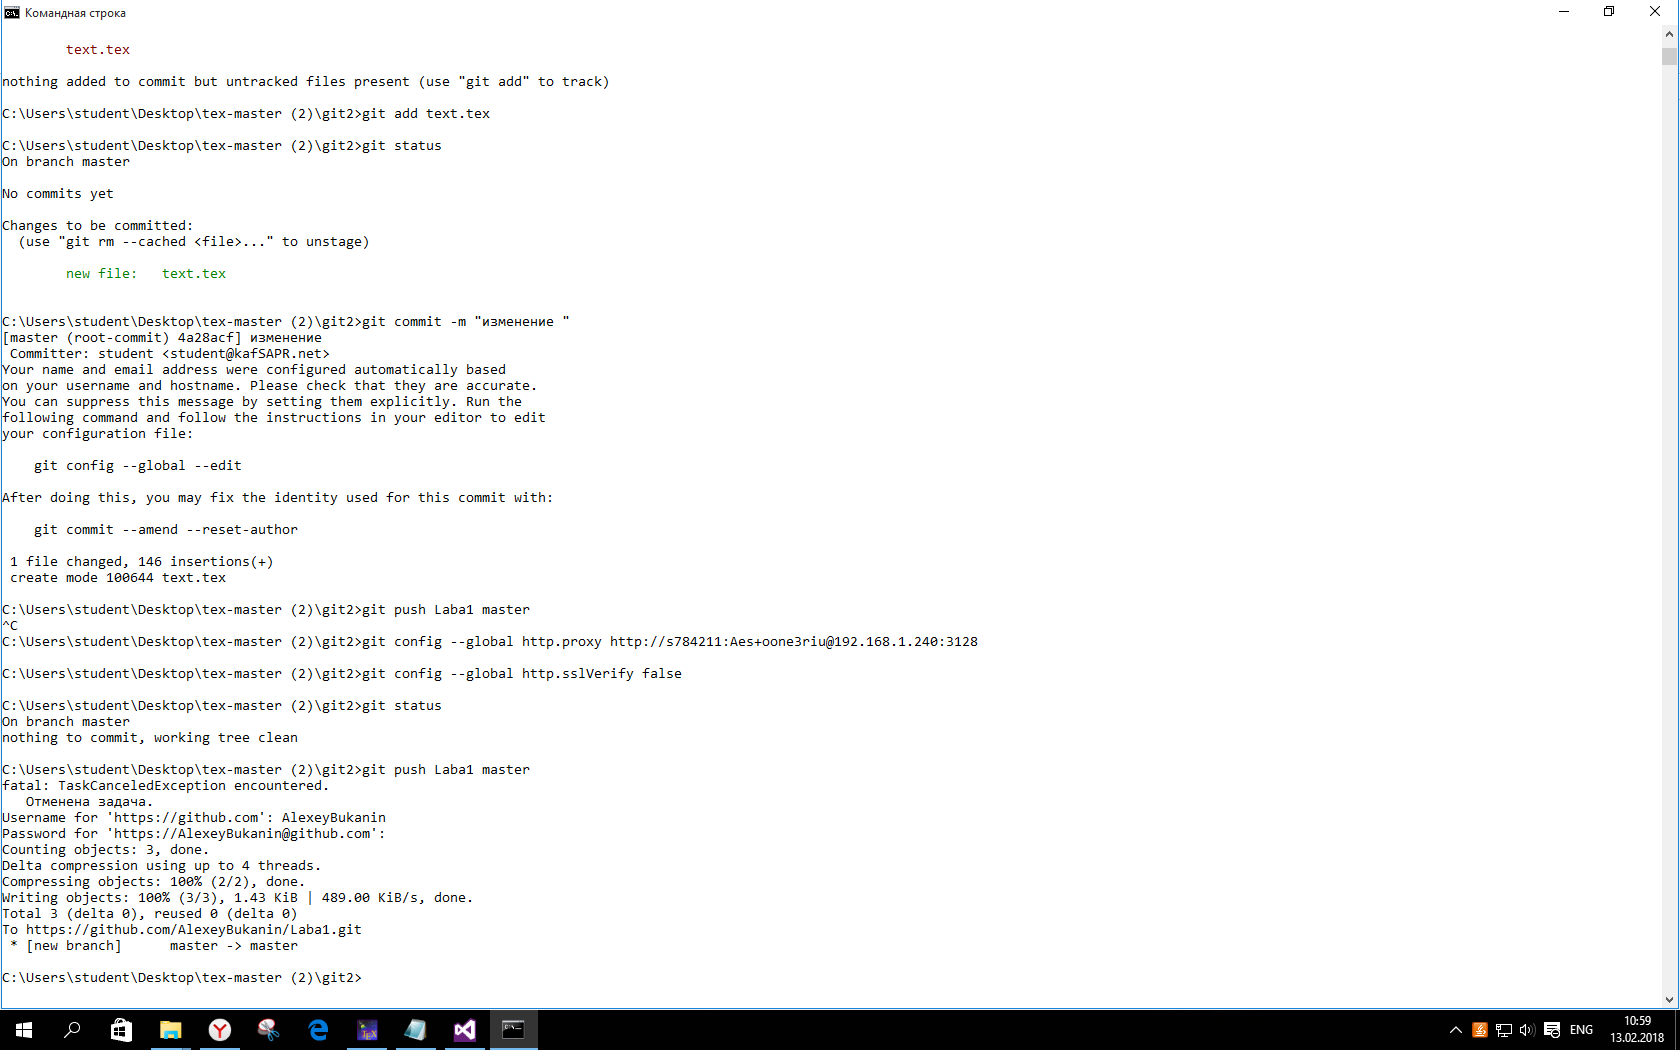
\includegraphics[scale=0.4]{com}
\caption{Используемые команды}
\label{fig:com}
\end{figure}

\newpage

\begin{figure}[h]
\centering
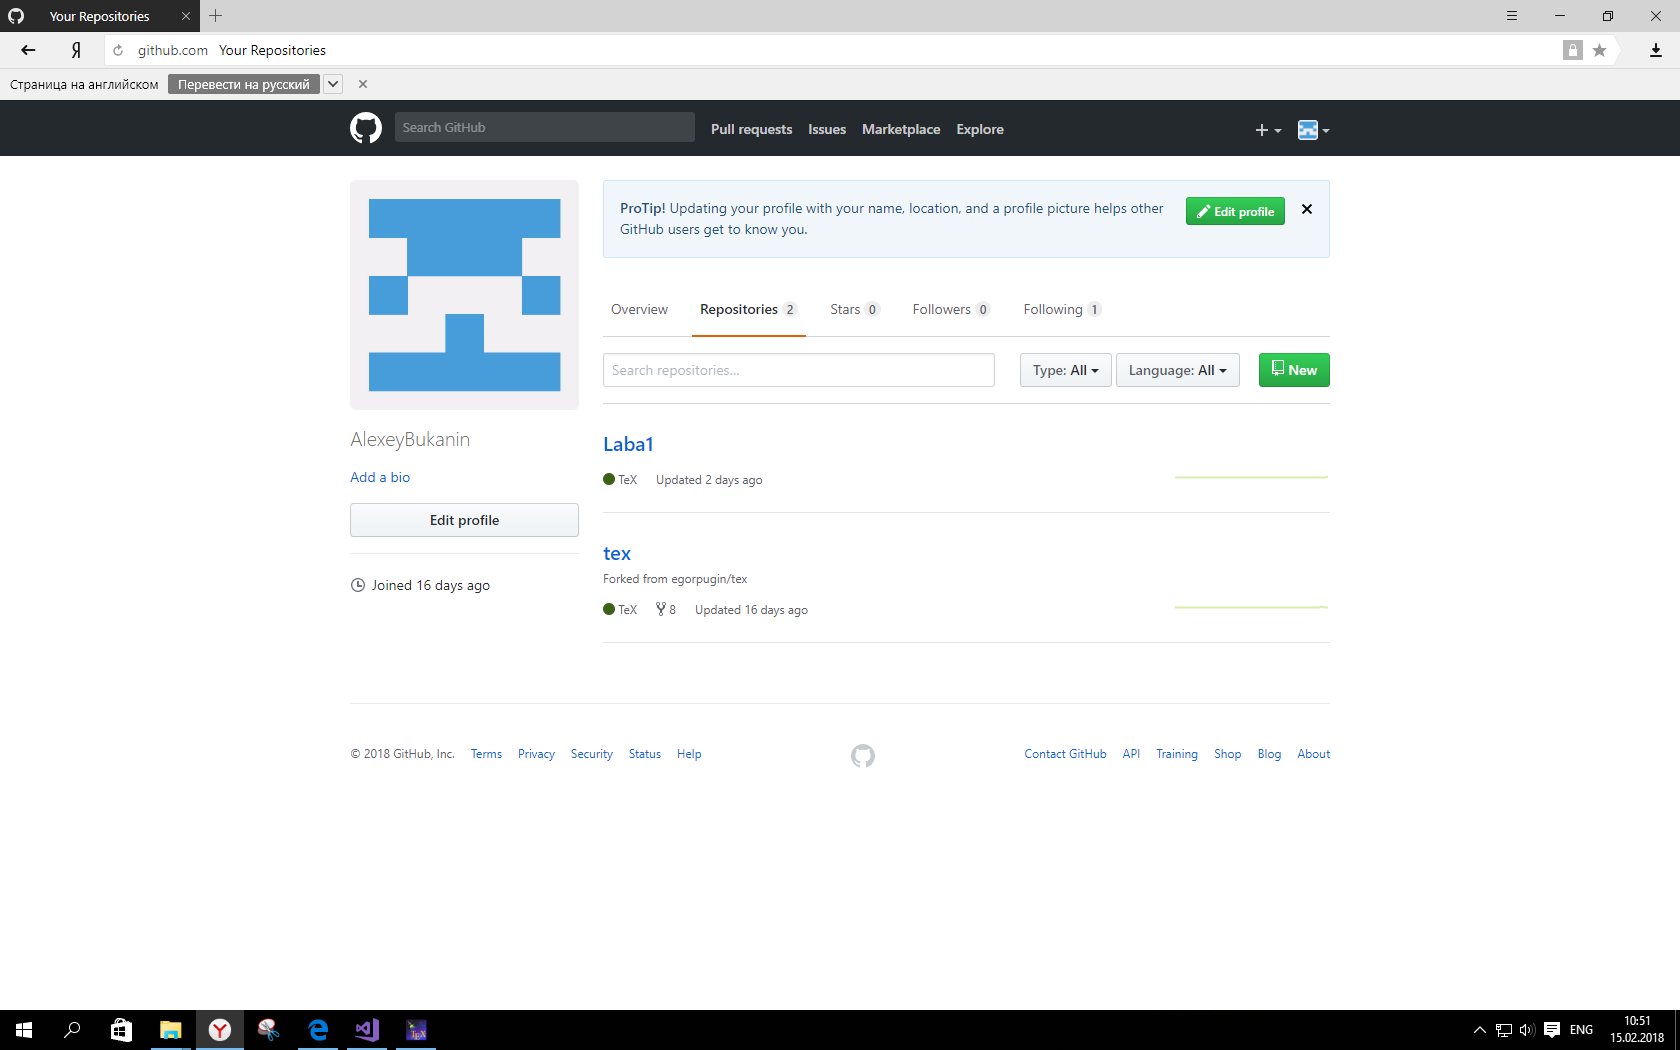
\includegraphics[scale=0.4]{Безымянный}
\caption{Результат}
\label{fig:Безымянный}
\end{figure}



\textbf{Вывод:} Я научился работать с gitom




\newpage

% Список литературы
\input{src/bibliography.tex}
\end{document}